\documentclass[a4paper]{article}

\usepackage[french]{babel}
\usepackage[utf8]{inputenc}
\usepackage{graphicx}
\usepackage{pdfpages}

\title{Small World : Rapport de Modélisation \\ INSA de Rennes - 4INFO}

\author{Axel CARO, Maximilien RICHER}

\date{\today}

\begin{document}
\maketitle

\paragraph{}
Ce document présente les résultats de la phase de modélisation du projet de quatrième année proposé en enseignement de \textit{Programmation et Modélisation orientées objet}.

\newpage

\section*{Introduction}
\paragraph{}
Le projet proposé consiste en la réalisation d'un jeu vidéo tour par tour, basé sur le jeu de plateau \textit{SmallWorld}. Au cours d'une partie, les joueurs s'affrontent pendant un certain nombre de tours, afin prendre le contrôle d'un territoire. Ce projet met l'accent sur les différentes phases de la réalisation d'un projet d'application orientée objet. La modélisation, l'utilisation de patrons de conceptions, l'organisation du code, l'implémentation, l'utilisation de librairies dynamiques, l'interfaçage entre plusieurs langages, la gestion d'IHM et les phases de tests sont des points clés des objectifs pédagogiques de ce projet.

\section{Présentation des règles du jeu}

\subsection{But du jeu}
\paragraph{}
Le but de SmallWorld est d'accumuler des points.
À la fin de chaque tour de jeu, le joueur compte les points gagnés et les ajoutes à son total. Au bout d'un nombre de tour défini au préalable, le jeu s'arrête et le joueur ayant le plus de point remporte la partie. Une partie peut également s'interrompre si un des joueurs élimine l'ensemble des unités de l'adversaire. Un joueur qui ne possède plus d'unités perd la partie, quel que soit son total de point.

\paragraph{}
\textbf{Déroulement d'une partie}
\begin{itemize}
    \item Choix de la configuration du plateau de jeu
    \item Choix des races
    \item Choix du joueur qui commence la partie
    \item Création du plateau de jeu
    \item Début du premier tour de jeu\\(\dots)
    \item Fin du dernier tour de jeu
    \item Décompte final des points
\end{itemize}

\subsubsection{Plateau de jeu}
\paragraph{}
Le jeu se déroule sur une plateau quadrillé de cases carré dont la dimension dépend du nombre de joueurs et de la durée de la partie.\label{map_gen} Il est composé de cases de différents types : plaine, mer, montagne et forêt.La carte est généré de manière aléatoire, mais doit contenir le même nombre de case de chaque type.

\subsubsection{Unité}
\paragraph{}
Des unitées sont placées sur le plateau, sur lequel elles peuvent se déplacer.

\subsubsection{Races et comptage des points en fin de tour}
E
\paragraph{}
\textbf{Configurations conseillées}
\begin{itemize}
    \item 2 joueurs, plateau de 6 par 6, 5 tours de jeu : 4 unités par joueur
    \item 2 joueurs, plateau de 10 par 10, 20 tours de jeu : 6 unités par joueur
    \item 2 joueurs, plateau de 14 par 14, 30 tours de jeu : 8 unités par joueur
\end{itemize}

\subsubsection{Préparation}
\paragraph{}
La préparation du jeu necéssite que le joueur choississe le type de partie parmis les configurations proposées, 

\subsection{Déroulement d'un tour de jeu}
\paragraph{}
Chaque \em{tour de jeu} est constitué de plusieurs \em{tours de joueurs}. Ces tours sont séquentiels. Lors du premier tour de jeu, le joueur jouant le premier tout est tiré au hasard, et cet ordre est conservé durant le reste de la partie.
\paragraph{}
\textbf{Déroulement du tour}
\begin{itemize}
    \item Début du tour
    \item Déplacement des unités et combats
    \item Décompte des points
    \item Fin du tour
\end{itemize}

\subsection{Déplacement et combat}


\section{Modélisation UML}
\paragraph{}
La phase de modélisation nous a conduit à réaliser plusieurs diagrammes UML, afin de représenter différents aspects de notre application. Nous présentons ci-après ces diagrammes, en explicitant leur contenu.

\subsection{Diagramme de paquetage}
\paragraph{}
Le diagramme suivant illustre la structuration à gros grain du code de notre application. On y retrouve les classes et interfaces que nous détaillerons dans la section \ref{DDC}.
Comme on peut le constater, nous n'avons pas hierarchisé notre application selon plusieurs paquetages. En effet, les interactions entre nos classes et interfaces auraient conduit à des dépendances circulaires entre les éventuels paquetages, mais transformer le modèle afin d'éviter ces problèmes aurait résulté en une complexité des traitements beaucoup plus importante, ou en la création de trop nombreux paquetages. Nous avons donc opté pour la simplicité de traitement. Les différentes classes et interfaces étant toutes liées, il nous semble inapproprié de les séparer dans des paquetages différents : les modifications éventuelles impacteront bon nombre d'entre elles, touchant à plusieurs des paquetages envisagés.

\paragraph{}
Par ailleurs, la séparation de notre application en paquetages "modèle" , "API" n'est pas pertinente, car ce projet ne porte que sur \textbf{une} implémentation du jeu proposé. Si plusieurs implémentations avaient été requises, la séparation précédente aurait alors eu du sens.

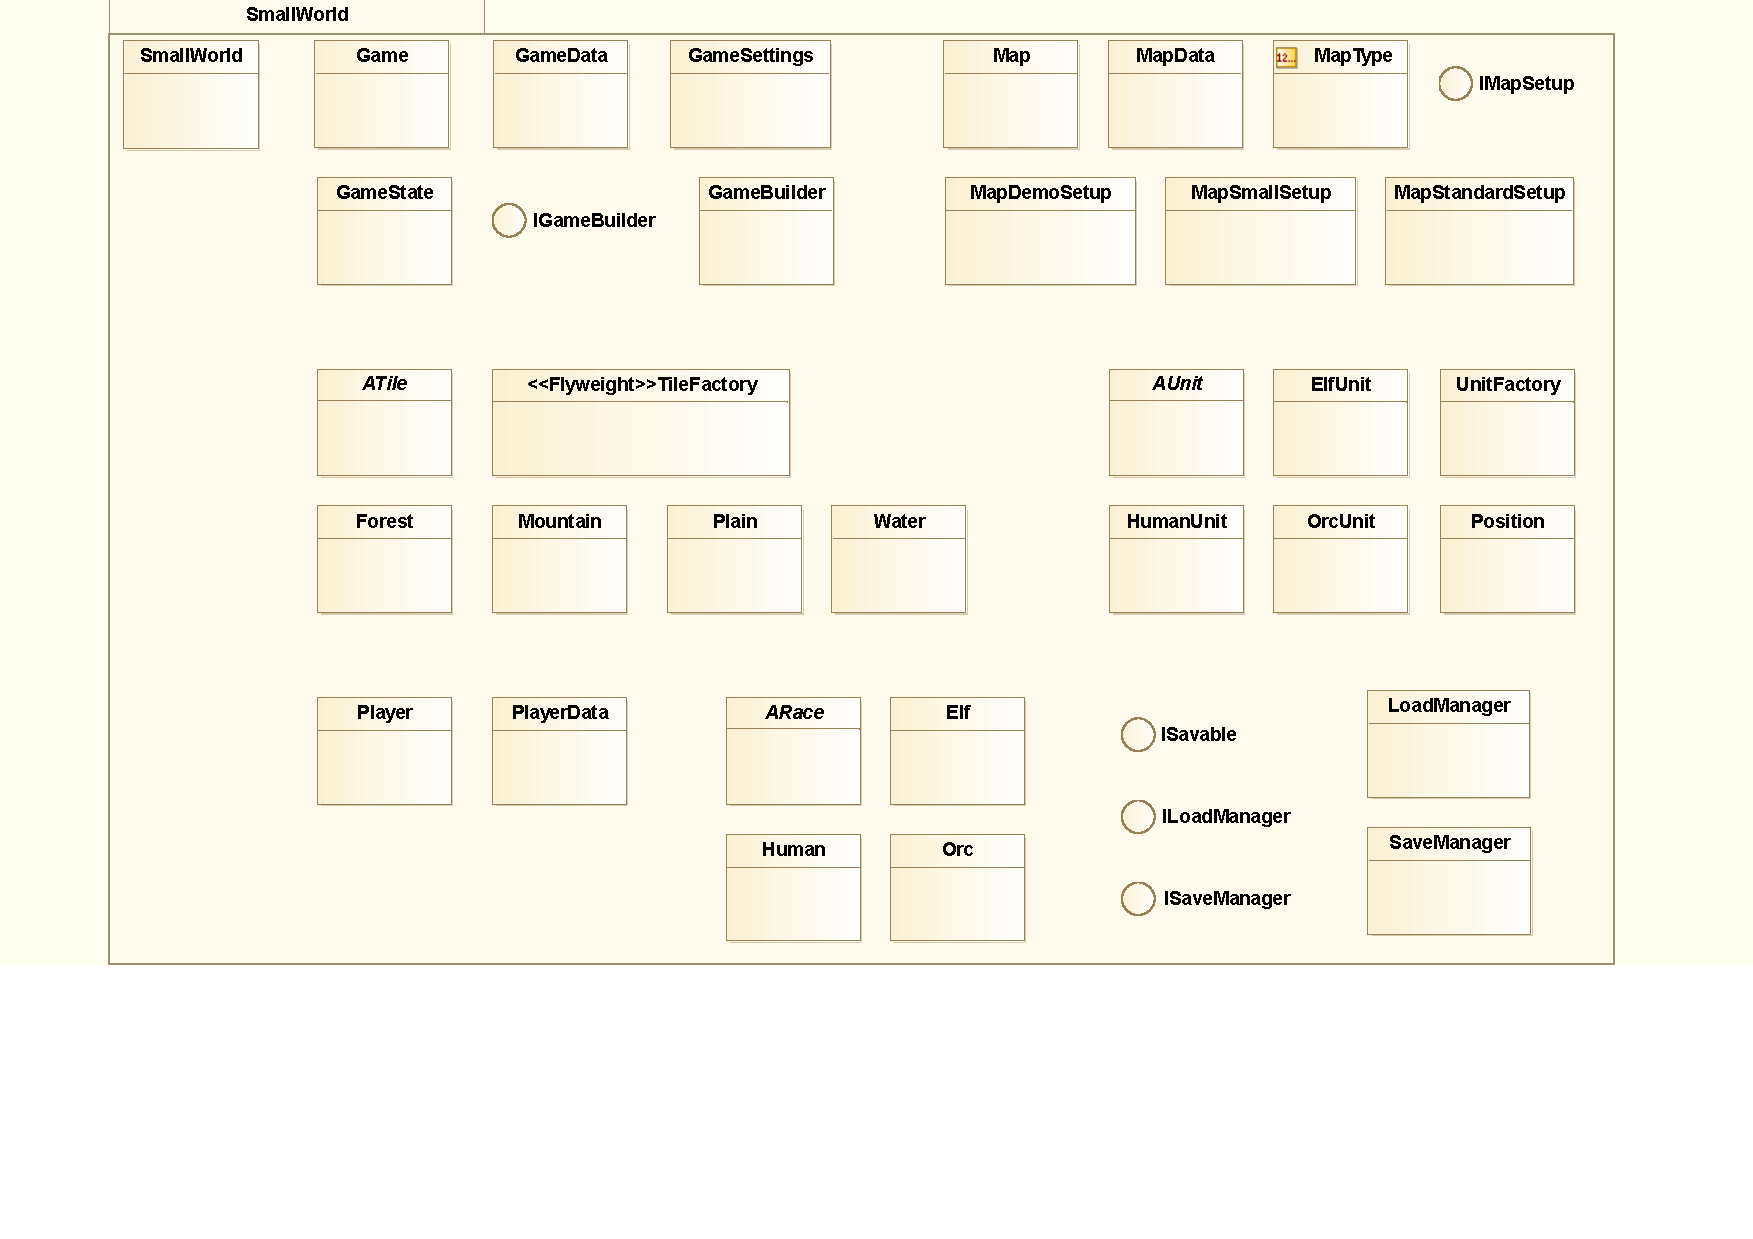
\includepdf[landscape=true]{images/packageDiagram.pdf}

\subsection{Diagramme de classes}
\label{DDC}
\paragraph{}
Le diagramme suivant illustre l'organisation en classes de notre application.

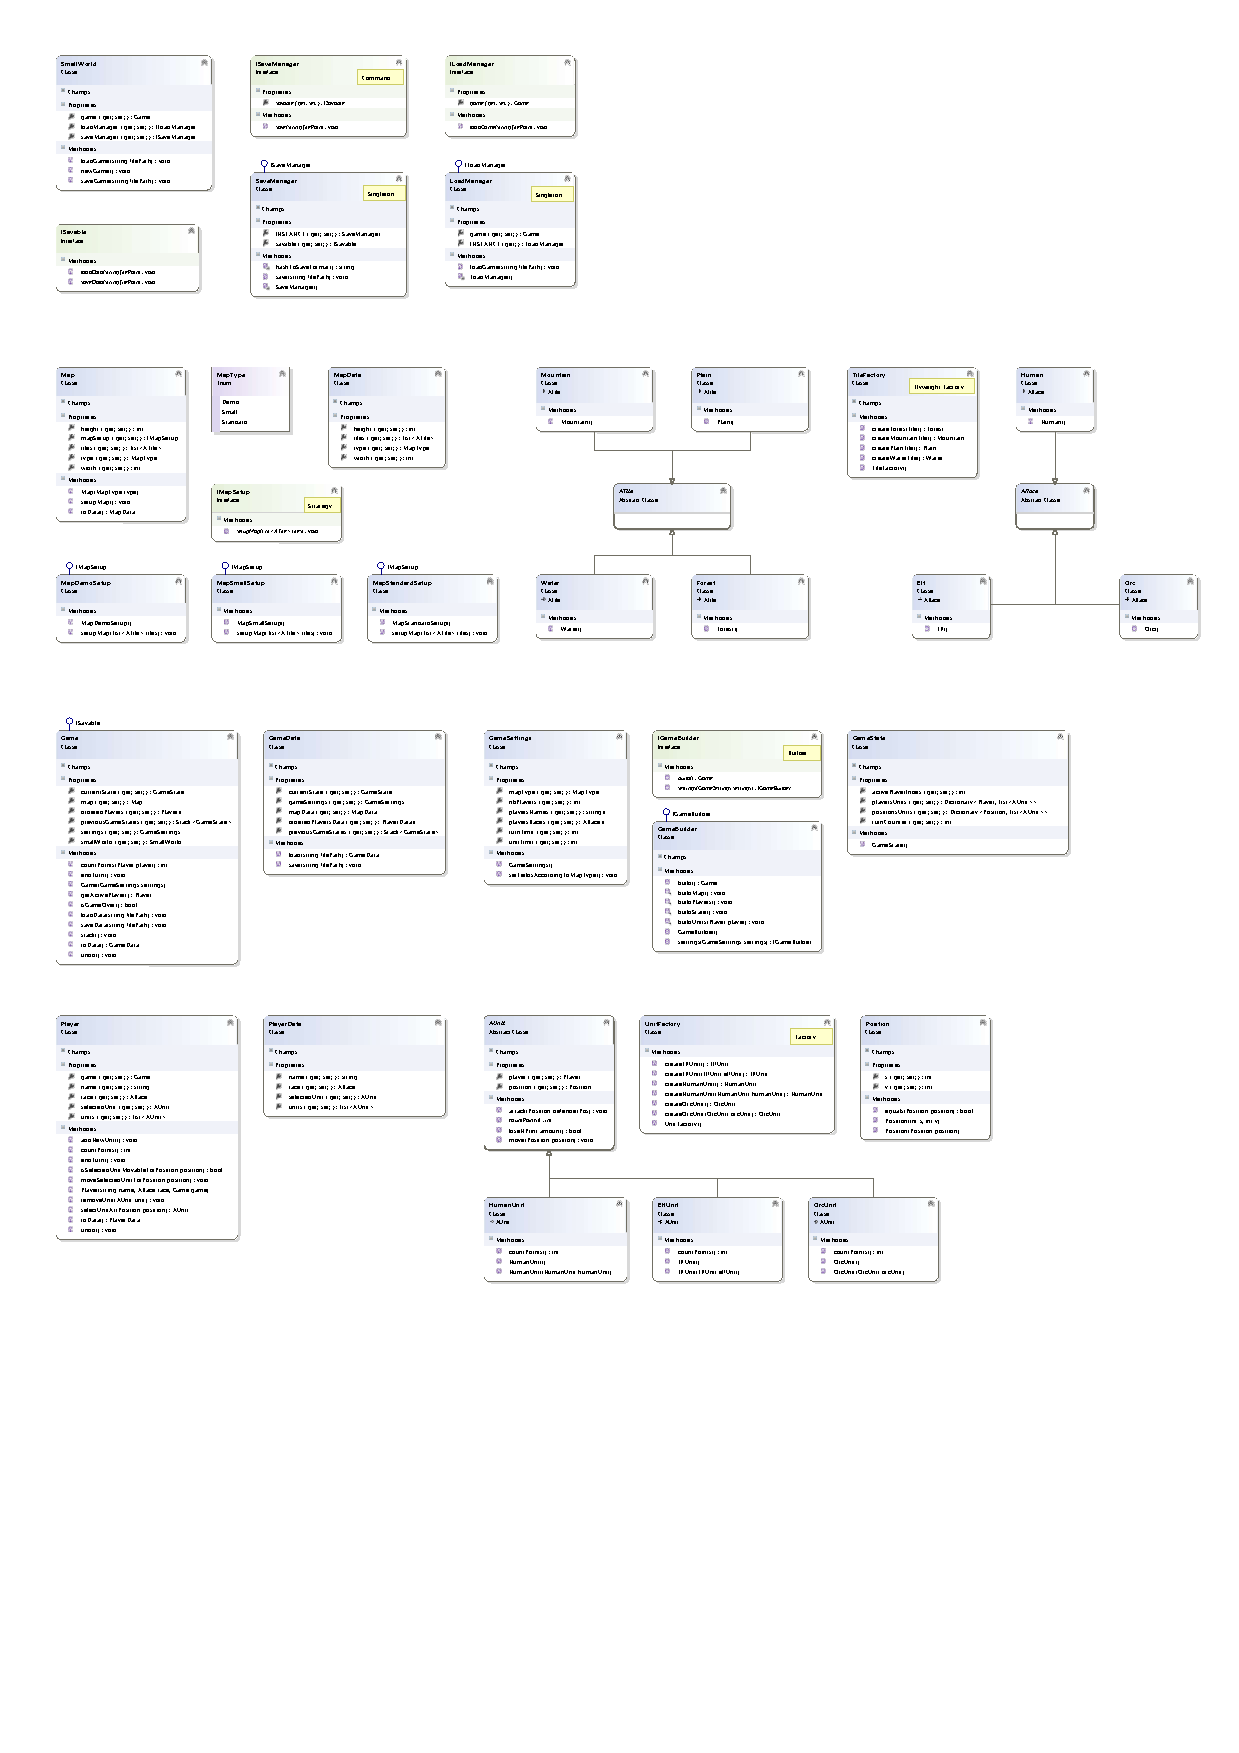
\includepdf{images/classDiagram.pdf}

\subsection{Diagrammes d'interaction}

\subsubsection{Diagramme de séquence : initialisation d'une partie}

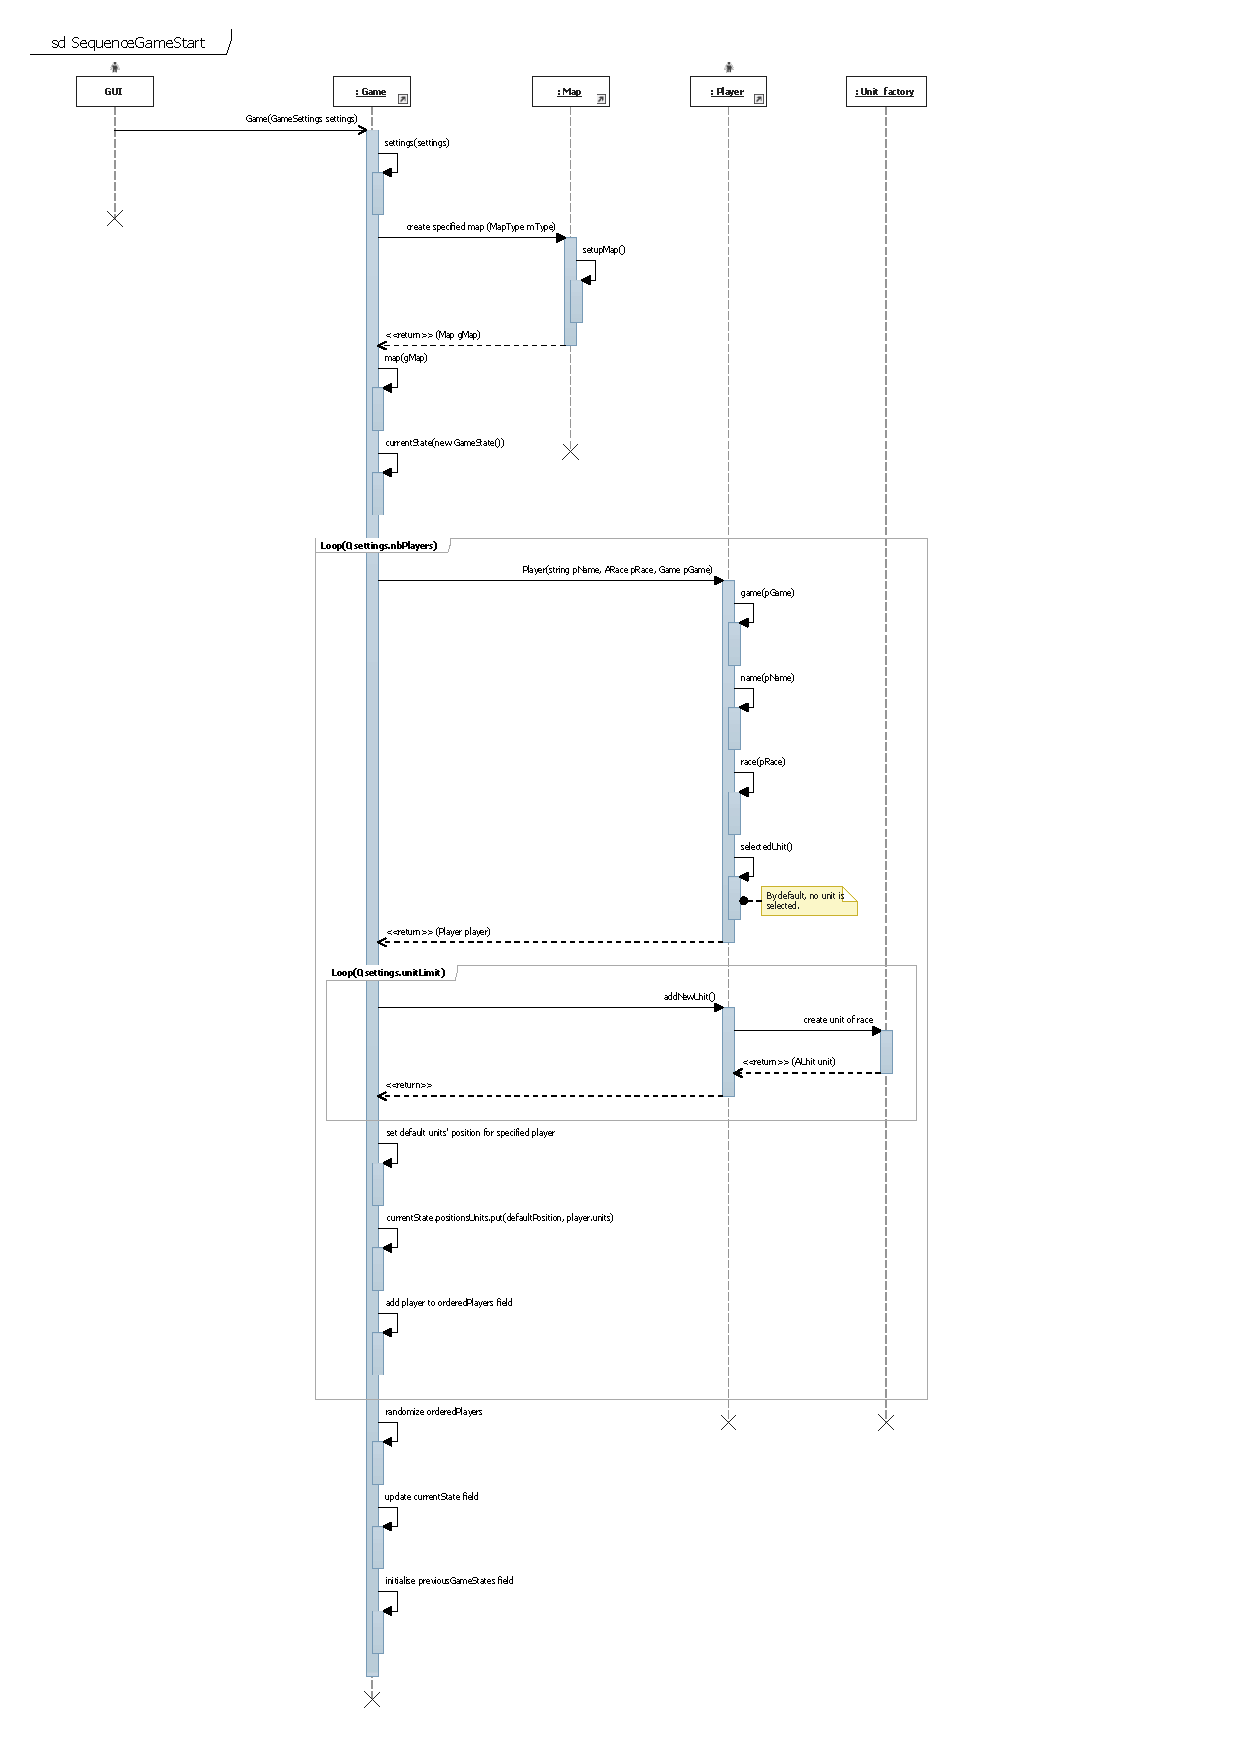
\includepdf{images/gameInitialisationSequenceDiagram.pdf}

\subsubsection{Diagramme de séquence : déroulement d'un tour}

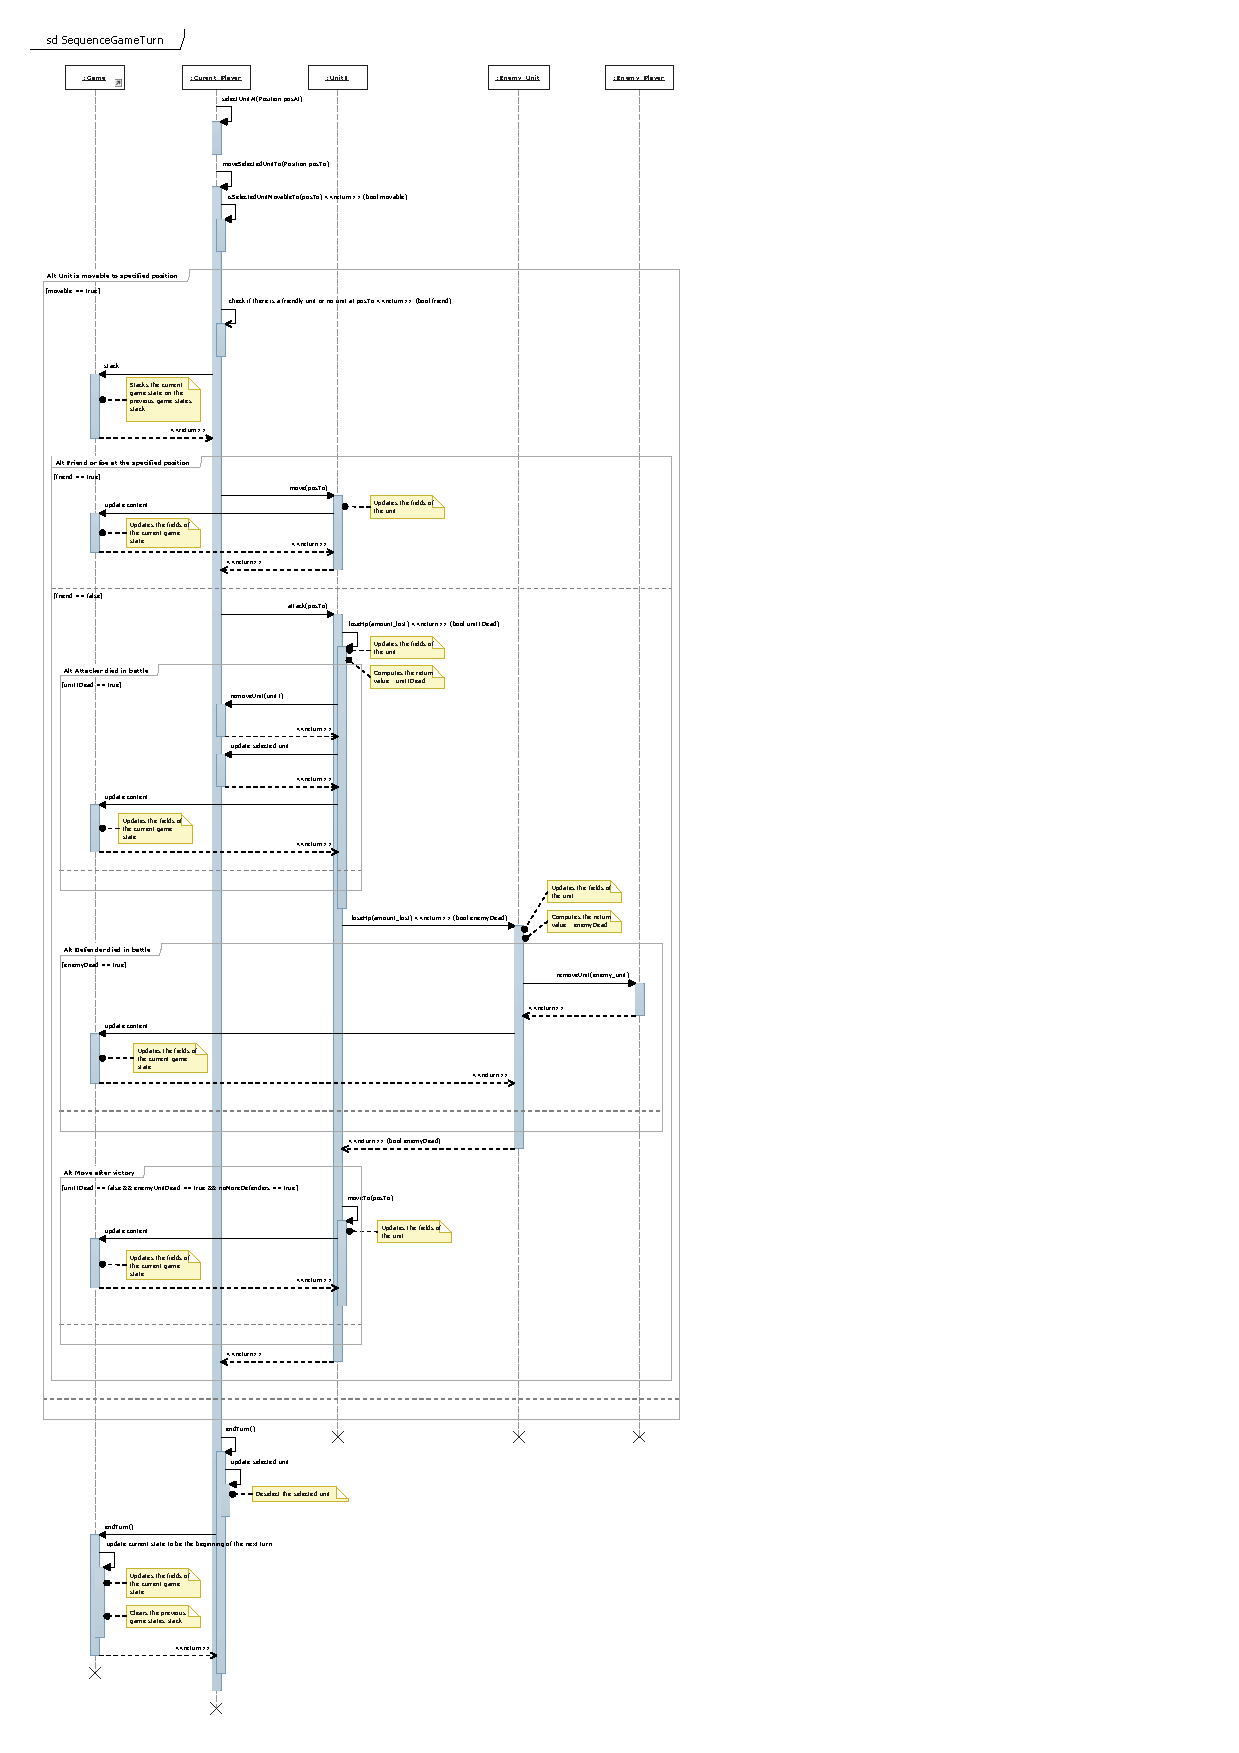
\includepdf{images/gameTurnSequenceDiagram.pdf}

\subsection{Diagramme d'états-transitions : gestion d'une unité}
Le diagramme suivant illustre les différents états d'une partie, et les évènements et conditions qui permettent une transition entre états.

\paragraph{}
En premier lieu, l'utilisateur détermine les paramètres de la partie (noms des joueurs, races, type de carte), puis ces informations sont transmises à la partie qui est alors \textbf{paramétrée}. La partie s'\textbf{initialise} alors selon les paramètres fournis. Durant cette phase, on détermine le joueur qui sera le premier à agir. La partie démarre alors un nouveau tour, et donne la main au premier joueur, que nous appellerons par la suite joueur 1.

\paragraph{}
Le changement de joueur s'effectue lors de l'annonce de fin de tour par le joueur 1. Si durant son tour, le joueur 1 est parvenu à éliminer toutes les unités de son adversaire, on arrive à la \textbf{victoire du joueur 1}. Si le joueur 1 a perdu toutes ses unités durant son tour et décide tout de même de le valider, on arrive à la \textbf{victoire du joueur 2}. Sinon, le jeu donne la main au joueur 2. De la même façon, on détermine si le joueur 2 gagne ou perd par élimination à la fin de son tour. On arrive alors à la \textbf{fin du tour de jeu} (tous les joueurs ont eu leur tour). S'il reste des tours à jouer, la partie donne la main au joueur 1.

\paragramh{}
À la fin du nombre limite de tours, si aucun des joueurs n'a atteint de victoire par élimination, on arrive à la \textbf{fin de partie}. La partie détermine alors, en fonction des points de victoire accumulés par les deux joueurs, s'il s'agit d'une situation de \textbf{victoire du joueur 1}, de \textbf{victoire du joueur 2}, ou encore d'\textbf{égalité}. La partie se termine alors.

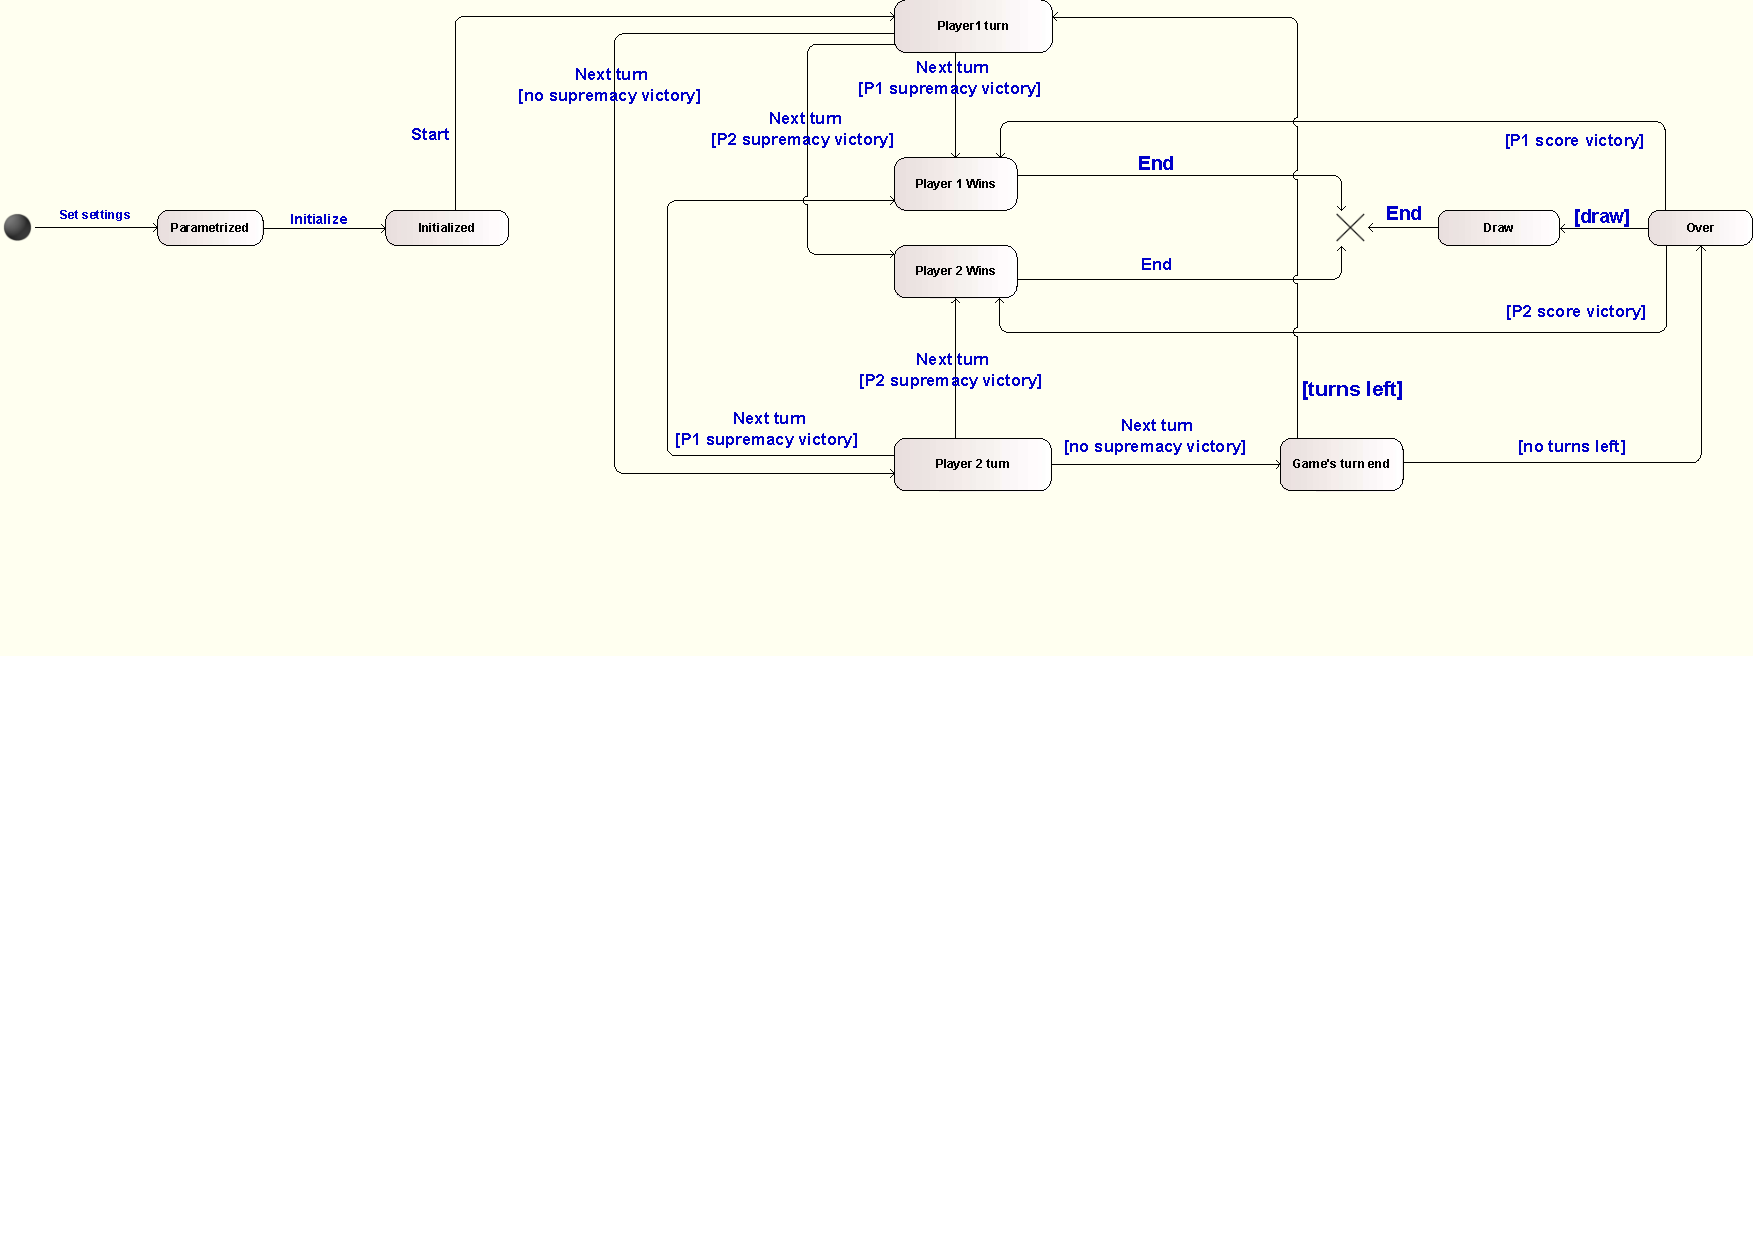
\includepdf{images/gameStatechart.pdf}

\end{document}
